\documentclass[aspectratio=169, 10pt]{beamer}

\usepackage{bm} % bold math
\usepackage{fontspec}
\usepackage{minted}
\usepackage{pgf-pie}
\usepackage{tikz}

% Custom commands and environments
\makeatletter
\newcommand\version[1]{\renewcommand\@version{#1}}
\newcommand\@version{}
\def\insertversion{\@version}

\newcommand\course[1]{\renewcommand\@course{#1}}
\newcommand\@course{}
\def\insertcourse{\@course}

\newcommand\coursetitle[1]{\renewcommand\@coursetitle{#1}}
\newcommand\@coursetitle{}
\def\insertcoursetitle{\@coursetitle}

\newcommand\lecturenumber[1]{\renewcommand\@lecturenumber{#1}}
\newcommand\@lecturenumber{}
\def\insertlecturenumber{\@lecturenumber}
\makeatother

\newcommand{\slidetitle}[1]{{\xbseries \large \structure{#1}} \bigskip}
\newcommand{\term}[1]{{\color{blue} #1}}
\newcommand{\leftspace}{\hspace{1em}}
\newcommand{\inlinearrow}{
  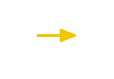
\begin{tikzpicture}[baseline]
    \node [anchor=base] (x) {};
    \draw [rawarrow] (x.mid west) -- ($(x.mid west) + (2em,0)$);
  \end{tikzpicture}
}

\newenvironment{slide}
{\begin{frame}[fragile,environment=slide]\vskip0pt plus 1filll}
{\vskip0pt plus 1filll\end{frame}}

% LaTeX

\setlength{\leftmargini}{1em}

% Common Information

\author{Jon Eyolfson}
\course{ECE 353}
\coursetitle{Systems Software}
\date{2024 Winter}

% fontspec

\defaultfontfeatures{Ligatures=TeX}
% \setmainfont{Domine}
\setsansfont{Inter}[
  FontFace={ul}{n}{Font=*-Thin},
  FontFace={el}{n}{Font=*-ExtraLight},
  FontFace={l}{n}{Font=*-Light},
  FontFace={sb}{n}{Font=*-SemiBold},
  FontFace={eb}{n}{Font=*-ExtraBold},
  FontFace={xb}{n}{Font=*-Black},
]
\setmonofont[Contextuals=AlternateOff, Ligatures=TeXOff]{Iosevka}[
  FontFace={xb}{n}{Font=*-Heavy},
]

%% Font Weights

\DeclareRobustCommand{\ulseries}{\fontseries{ul}\selectfont}
\DeclareTextFontCommand{\textul}{\ulseries}
\DeclareRobustCommand{\elseries}{\fontseries{el}\selectfont}
\DeclareTextFontCommand{\textel}{\elseries}
\DeclareRobustCommand{\lseries}{\fontseries{l}\selectfont}
\DeclareTextFontCommand{\textl}{\lseries}
\DeclareRobustCommand{\sbseries}{\fontseries{sb}\selectfont}
\DeclareTextFontCommand{\textsb}{\sbseries}
\DeclareRobustCommand{\ebseries}{\fontseries{eb}\selectfont}
\DeclareTextFontCommand{\texteb}{\ebseries}
\DeclareRobustCommand{\xbseries}{\fontseries{xb}\selectfont}
\DeclareTextFontCommand{\textxb}{\xbseries}

% tikz

\usetikzlibrary{
  arrows,
  arrows.meta,
  automata,
  backgrounds,
  calc,
  decorations.pathreplacing,
  matrix,
  positioning,
  overlay-beamer-styles,
  shapes,
  shapes.multipart,
  tikzmark,
}

\tikzstyle{rawarrow} = [
  -{Latex[round]},
  line width=1pt,
  yellow,
  shorten >=3pt,
  shorten <=3pt,
  font=\small,
  text=black,
]

\tikzstyle{arrow} = [
  -{Latex[round]},
  line width=1pt,
  yellow,
  shorten >=3pt,
  shorten <=3pt,
  transform canvas={yshift=3pt},
  font=\small,
  text=black,
]

\newcommand{\tikzmarkcoord}[1]{([yshift=3pt]pic cs:#1)}

% minted

\setminted{style=eyolfson, fontsize=\small, escapeinside=||}
\setmintedinline{fontsize=\normalsize}

% hyperref

\hypersetup{colorlinks, urlcolor=blue}

% beamer
\setbeamersize{text margin left=16mm, text margin right=16mm}
\setbeamertemplate{itemize items}[circle]
\setbeamercolor{item}{fg=black}
\setbeamercolor{structure}{fg=darkblue}
\setbeamerfont{frametitle}{series=\bfseries, parent=structure}
\setbeamertemplate{navigation symbols}{}
\setbeamertemplate{headline}{}
\setbeamertemplate{footline}{
  \begin{tikzpicture}[
    remember picture,
    overlay,
    shift={(current page.south west)},
  ]
    \path [fill=gray] (144mm, 0) -- (160mm, 16mm) -- (160mm, 0);
    \node [inner sep=3.5mm, outer sep=0, text=black, anchor=base east,
           align=right, yshift=3.5mm]
          at (current page.south east) {\ttfamily \small \insertframenumber{}};
  \end{tikzpicture}
}
\setbeamertemplate{title page}{
  \begin{tikzpicture}[
    remember picture,
    overlay,
    shift={(current page.south west)},
    background rectangle/.style={fill=darkblue},
    show background rectangle,
  ]
    \node [anchor=center, align=center, text=white, text width=40mm, scale=3.2]
          at (\paperwidth / 2, \paperheight * 2 / 3)
          {\xbseries \inserttitle{}};
    \node [anchor=base west, align=left, inner sep=0, text=white, yshift=2.5mm]
          at (16mm, \paperheight / 3)
          {\insertdate{} \insertcourse{}: \insertcoursetitle{}};
    \node [anchor=base west, align=left, inner sep=0, text=white, yshift=-2.5mm]
          at (16mm, \paperheight / 3)
          {\insertauthor};
    \node [anchor=base east, align=right, inner sep=0, text=white, yshift=2.5mm]
          at (144mm, \paperheight / 3)
          {Lecture \insertlecturenumber{}};
    \node [anchor=base east, align=right, inner sep=0, text=white,
           yshift=-2.5mm]
          at (144mm, \paperheight / 3)
          {\ttfamily \insertversion{}};
    \node [align=center, anchor=south, inner sep=0, text=white, yshift=3.5mm]
          (license) at (\paperwidth / 2, 0)
          {\fontsize{7pt}{7pt}\selectfont This  work is licensed under a
           \href{http://creativecommons.org/licenses/by-sa/4.0/}
                {\color{lightblue} Creative Commons Attribution-ShareAlike 4.0
                 International License}};
  \end{tikzpicture}
}

% xcolor

%% Primary Colour

\definecolor{pantone655}{RGB}{0, 42, 92} % #002a5c
\colorlet{darkblue}{pantone655}

%% Secondary Colours

\definecolor{pantone633}{RGB}{0, 139, 176} % #008bb0
\colorlet{blue}{pantone633}

\definecolor{pantonewarmred}{RGB}{220, 70, 51} % #dc4633
\colorlet{red}{pantonewarmred}

\definecolor{pantone3285}{RGB}{0, 161, 137} % #00a189
\colorlet{cyan}{pantone3285}

\definecolor{pantone7722}{RGB}{13, 83, 77} % #0d534d
\colorlet{darkcyan}{pantone7722}

\definecolor{pantone376}{RGB}{141, 191, 46} % #8dbf2e
\colorlet{green}{pantone376}

\definecolor{pantone2613}{RGB}{109, 36, 122} % #6d247a
\colorlet{violet}{pantone2613}

\definecolor{pantone2985}{RGB}{111, 199, 234} % #6fc7ea
\colorlet{lightblue}{pantone2985}

\definecolor{pantone227}{RGB}{171, 19, 104} % #ab1368
\colorlet{magenta}{pantone227}

\definecolor{pantone7406}{RGB}{241, 197, 0} % #f1c500
\colorlet{yellow}{pantone7406}

%% Neutrals

\definecolor{pantonecoolgray2}{RGB}{208, 209, 201} % #d0d1c9
\colorlet{gray}{pantonecoolgray2}


\lecturenumber{2}
\title{Kernels}
\version{2.0.0}

\begin{document}

\begin{frame}[plain, noframenumbering]
  \titlepage
\end{frame}

\begin{slide}
  \slidetitle{Let's Execute This Program and Verify It's ``Hello world''}

  \small \ttfamily
  0x7F 0x45 0x4C 0x46 0x02 0x01 0x01 0x00 0x00 0x00 0x00 0x00 0x00 0x00 0x00
  0x00

  0x02 0x00 0xB7 0x00 0x01 0x00 0x00 0x00 0x78 0x00 0x01 0x00 0x00 0x00 0x00
  0x00

  0x40 0x00 0x00 0x00 0x00 0x00 0x00 0x00 0x00 0x00 0x00 0x00 0x00 0x00 0x00
  0x00

  0x00 0x00 0x00 0x00 0x40 0x00 0x38 0x00 0x01 0x00 0x40 0x00 0x00 0x00 0x00
  0x00

  0x01 0x00 0x00 0x00 0x05 0x00 0x00 0x00 0x00 0x00 0x00 0x00 0x00 0x00 0x00
  0x00

  0x00 0x00 0x01 0x00 0x00 0x00 0x00 0x00 0x00 0x00 0x01 0x00 0x00 0x00 0x00
  0x00

  0xA8 0x00 0x00 0x00 0x00 0x00 0x00 0x00 0xA8 0x00 0x00 0x00 0x00 0x00 0x00
  0x00

  0x00 0x10 0x00 0x00 0x00 0x00 0x00 0x00 0x08 0x08 0x80 0xD2 0x20 0x00 0x80
  0xD2

  0x81 0x13 0x80 0xD2 0x21 0x00 0xA0 0xF2 0x82 0x01 0x80 0xD2 0x01 0x00 0x00
  0xD4

  0xC8 0x0B 0x80 0xD2 0x00 0x00 0x80 0xD2 0x01 0x00 0x00 0xD4 0x48 0x65 0x6C
  0x6C

  0x6F 0x20 0x77 0x6F 0x72 0x6C 0x64 0x0A
  \bigskip

  \normalsize \normalfont Execute using:
  \mintinline{bash}{./hello-world-linux-aarch64}
\end{slide}

\begin{slide}
  
  \slidetitle{Aside: There's 3 Major ISAs in Use Today}

  ISA stands for the \textit{instruction set architecture}

  \leftspace{} It's the machine code, or numbers the CPU understands
  \bigskip

  \texttt{x86-64} (aka \texttt{amd64}): for desktops, non-Apple laptops,
                                          servers
  \medskip

  \texttt{aarch64} (aka \texttt{arm64}): for phones, tablets, Apple laptops
  \medskip

  \texttt{riscv} (aka \texttt{rv64gc}): open-source implementation, similar to
                                        ARM
  \bigskip

  We'll touch on all of them in this course
\end{slide}

\begin{slide}
  
  \slidetitle{Our Next Abstraction is a File Descriptor}

  Since our processes are independent, we need an explicit way to transfer data
  \medskip

  \textbf{IPC:} inter-process communication is transferring data between two
  processes
  \bigskip

  \textbf{File descriptor:} a resource that users may either read bytes from
  or write bytes to \newline
  (identified by an index stored in a process)
  \medskip

  A file descriptor could represent a file, or your terminal
\end{slide}

\begin{slide}
  
  \slidetitle{System Calls Make Requests to the Operating System}

    We can represent system calls like regular C functions
    \medskip

    Here are two system calls we need for a basic ``Hello world'' program:
    \bigskip

    \mintinline{c}{ssize_t write(int fd, const void *buf, size_t count);}

    \textbf{Description:} writes bytes from a byte array to a file descriptor

    \leftspace{}\mintinline{c}{fd} - the file descriptor

    \leftspace{}\mintinline{c}{buf} - the address of the start of the byte
    array (called a buffer)

    \leftspace{}\mintinline{c}{count} - how many bytes to write from the
    buffer
    \bigskip

    \mintinline{c}{void exit_group(int status);}

    \textbf{Description:} exits the current process and sets an exit status code

    \leftspace{}\mintinline{c}{status} - the exit status code (0-255)
\end{slide}

\begin{slide}
  
  \slidetitle{A Hypothetical ``Hello world'' Program}

  By convention there's some expected file descriptors:

  \leftspace{}\mintinline{c}{0} - standard input (read)

  \leftspace{}\mintinline{c}{1} - standard output (write)

  \leftspace{}\mintinline{c}{2} - standard error (write)
  \bigskip

  The most basic ``Hello world'' program would start executing the following:

  \begin{minted}{c}
void _start(void) {
  write(1, "Hello world\n", 12);
  exit_group(0);
}
  \end{minted}

\end{slide}

\begin{slide}
  
  \slidetitle{Another Aside: API Tells You What and ABI Tells You How} 

  Application Programming Interface (API) abstracts the details and describes
  the arguments and return value of a function
  \medskip

  \leftspace{}e.g. A function takes 2 integer arguments
  \bigskip

  Application Binary Interface (ABI) specifies the details, specifically how to
  pass arguments and where the return value is
  \medskip

  \leftspace{}e.g. The same function using the C calling convention
  
  \leftspace{}(arguments on the stack)
\end{slide}

\begin{slide}
  
  \slidetitle{System Call ABI for Linux AArch64}

  The operating system ``functions'' do not have an address,
  
  \leftspace{}instead we can generate an interrupt for the OS
  \bigskip

  Generate an interrupt with a \mintinline{nasm}{svc} instruction, using registers for
  arguments:

  \begin{itemize}
    \item \texttt{x8} --- System call number
    \item \texttt{x0} --- 1\textsuperscript{st} argument
    \item \texttt{x1} --- 2\textsuperscript{nd} argument
    \item \texttt{x2} --- 3\textsuperscript{rd} argument
    \item \texttt{x3} --- 4\textsuperscript{th} argument
    \item \texttt{x4} --- 5\textsuperscript{th} argument
    \item \texttt{x5} --- 6\textsuperscript{th} argument
  \end{itemize}
  \bigskip

  What are the limitations of this?
\end{slide}

\begin{slide}
  
  \slidetitle{Last Aside: C ABI, or Calling Convention for x86-64}

  System calls use registers, while C is stack based:

  \begin{itemize}
    \item Arguments pushed on the stack from right-to-left order
    \item \texttt{rax}, \texttt{rcx}, \texttt{rdx} are caller saved
    \item Remaining registers are callee saved
    \item Some arguments may be passed in registers instead of the stack
  \end{itemize}
  \medskip

  See \href{https://en.wikipedia.org/wiki/X86_calling_conventions}{Wikipedia}
  for more details (there's lots of conventions, think ECE 243)
  \bigskip

  What advantages does this give us vs system call ABI? Disadvantages?
\end{slide}

\begin{slide}
  
  \slidetitle{Programs on Linux Use the ELF File Format}

  Executable and Linkable Format (ELF) specifies both executables and libraries
  \medskip

  Always starts with the 4 bytes: \mintinline{text}{0x7F 0x45 0x4C 0x46}

  \leftspace{}or with ASCII encoding: \mintinline{text}{DEL 'E' 'L' 'F'}
  \medskip

  These 4 bytes are called ``magic'', and that's how you know what kind of file
  this is (other file formats may have a different number of bytes)
  \bigskip

  See: \url{https://en.wikipedia.org/wiki/List_of_file_signatures}

  \leftspace{}e.g., PDF files start with \mintinline{text}{%PDF-}
\end{slide}

\begin{slide}
  
  \slidetitle{Our Bytes Represent an ELF File}

  Tells the OS to load the entire executable file into memory at
  address \texttt{0x10000}
  \medskip

  The file header is 64 bytes, and the ``program header'' is 56 bytes

  (120 bytes total)
  \medskip

  The next 36 bytes are instructions, then 12 bytes for the string
  \mintinline{c}{"Hello world\n"}

  \leftspace{}Instructions start at \texttt{0x10078} (\texttt{0x78} is 120)

  \leftspace{}The string (data) starts at \texttt{0x1009C} (\texttt{0x9C} is 156)
  \medskip

  You can use: \mintinline{bash}{readelf -a <FILE>} to see the gory details
\end{slide}

\begin{slide}
  
  \slidetitle{Visually How Our ELF File Gets Divided}

  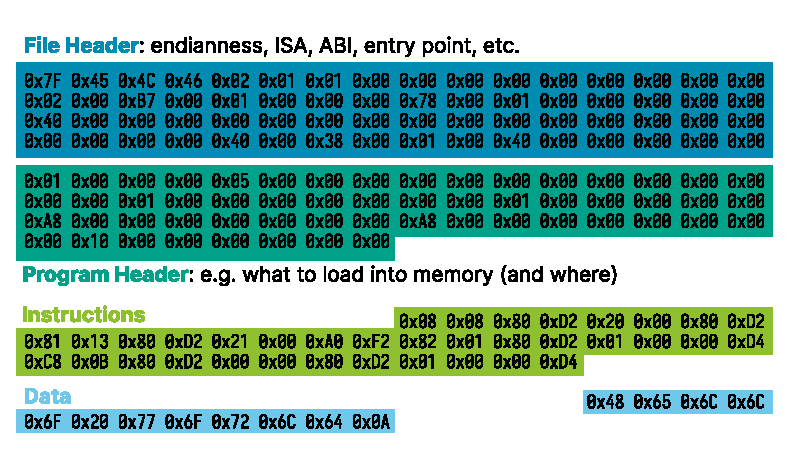
\includegraphics{hello-world-elf.eps}

\end{slide}

\begin{slide}
  
  \slidetitle{Instructions for ``Hello world'', Using the Linux AArch64 ABI}

  Plug in the 36 bytes for instructions into a disassembler, such as:
  \url{https://onlinedisassembler.com/}
  \bigskip

  Our disassembled instructions:
  \begin{minted}{nasm}
mov  x8, 0x40          #64
mov  x0, 0x01          #1
mov  x1, 0x9C          #156
movk x1, 0x01, lsl 16  #0x10000
mov  x2, 0x0C          #12
svc  0x0
mov  x8, 0x5E          # 94
mov  x0, 0x0           # 0
svc  0x0
  \end{minted}
\end{slide}

\begin{slide}
  
  \slidetitle{Data for Our ``Hello world'' Example}

  The 12 bytes of data is the \mintinline{c}{"Hello world"} string itself, ASCII
  encoded:

  \leftspace{}\texttt{\small 0x48 0x65 0x6C 0x6C 0x6F 0x20 0x77 0x6F 0x72 0x6C 0x64
                        0x0A}
  \medskip

  Low level ASCII tip: bit 5 is \texttt{0}/\texttt{1} for upper
  case/lower case (values differ by 32)
  \bigskip

  This accounts for every single byte of our 168 byte program, let's see what
  C does...
  \bigskip

  Can you already spot a difference between strings in our example compared to
  C?
\end{slide}

\begin{slide}
  
  \slidetitle{The Kernel is a Core Part of Your Operating System}

  \textbf{Kernel mode} is a privilege level on your CPU that gives access
  to more instructions
  \bigskip

  Different architectures have a different name for this mode

  \leftspace{}e.g., this is S-mode on RISC-V

  \bigskip
  \pause

  The kernel is the part of your operating system that runs in kernel mode
  \medskip

  These instructions allow only trusted software to interact with hardware

  \leftspace{}e.g., only the kernel can manage virtual memory for processes
\end{slide}

\begin{slide}
  
  \slidetitle{More Privileged CPU Modes Can Access More Instructions}

  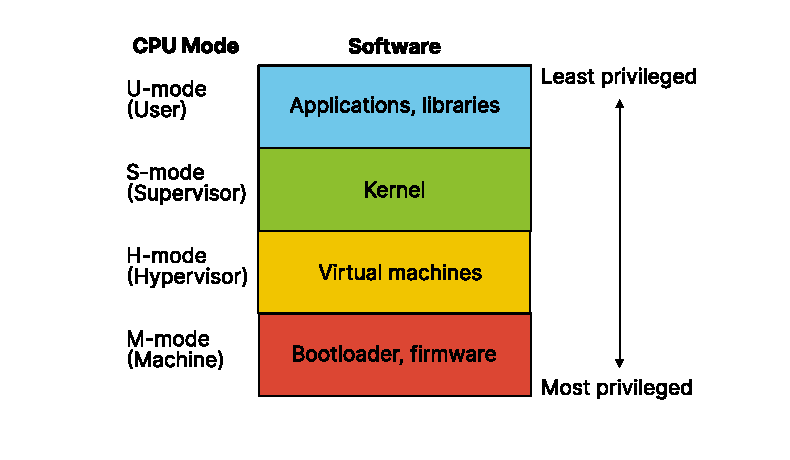
\includegraphics{cpu-modes.eps}

\end{slide}

\begin{slide}
  
  \slidetitle{System Calls Transition Between User and Kernel Mode}

  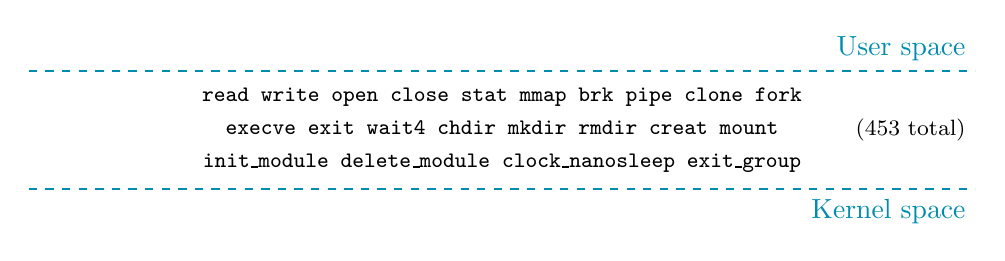
\begin{tikzpicture}
    \draw [blue, dashed, thick] (0,0.75)
                                        -- ($(\textwidth - 3pt, 0.75)$);
    \node [blue, anchor=south east] at ($(\textwidth - 3pt, 0.75)$)
          (user) {User space};
    \draw [blue, dashed, thick] (0,-0.75)
                                        -- ($(\textwidth - 3pt, -0.75)$);
    \node [blue, anchor=north east] at ($(\textwidth - 3pt, -0.75)$)
          (kernel) {Kernel space};
    \node [anchor=east] at ($(\textwidth - 3pt, -0)$)
          {\footnotesize (453 total)};
    \node [align=center] at ($(\textwidth/2 - 1.5pt, 0)$)
      {\footnotesize\ttfamily read write open close stat mmap brk pipe clone
                              fork \\
        \footnotesize\ttfamily execve exit wait4 chdir  mkdir rmdir creat mount
                              \\
        \footnotesize\ttfamily init\_module delete\_module clock\_nanosleep
                              exit\_group };
  \end{tikzpicture}
\end{slide}

\begin{slide}
  
  \slidetitle{System Calls Are Traceable}

  We can trace all the system calls a process makes on Linux using the command:

  \leftspace{}\mintinline{bash}{strace <PROGRAM>}
  \medskip

  We can see all the system calls our ``Hello world'' program makes:

  \begin{minted}{console}
execve("./hello_world", ["./hello_world"], 0x7ffd0489de40 /* 46 vars */) = 0
write(1, "Hello world\n", 12)           = 12
exit_group(0)                           = ?
+++ exited with 0 +++
  \end{minted}
  \bigskip

  Now, let's really see what C does...
\end{slide}

\begin{slide}

  \slidetitle{System Calls for ``Hello world'' in C, Finding Standard Library}

  \begin{minted}[fontsize=\scriptsize, escapeinside=]{console}
execve("./hello_world_c", ["./hello_world_c"], 0x7ffcb3444f60 /* 46 vars */) = 0
brk(NULL)                               = 0x5636ab9ea000
openat(AT_FDCWD, "/etc/ld.so.cache", O_RDONLY|O_CLOEXEC) = 3
fstat(3, {st_mode=S_IFREG|0644, st_size=149337, ...}) = 0
mmap(NULL, 149337, PROT_READ, MAP_PRIVATE, 3, 0) = 0x7f4d43846000
close(3)                                = 0
openat(AT_FDCWD, "/usr/lib/libc.so.6", O_RDONLY|O_CLOEXEC) = 3
read(3, "\177ELF\2\1\1\3\0\0\0\0\0\0\0\0\3\0>\0\1\0\0\0000C"..., 832) = 832
lseek(3, 792, SEEK_SET)                 = 792
read(3, "\4\0\0\0\24\0\0\0\3\0\0\0GNU\0\201\336\t\36\251c\324"..., 68) = 68
fstat(3, {st_mode=S_IFREG|0755, st_size=2136840, ...}) = 0
mmap(NULL, 8192, PROT_READ|PROT_WRITE, MAP_PRIVATE|MAP_ANONYMOUS, -1, 0) = 0x7f4d43844000
lseek(3, 792, SEEK_SET)                 = 792
read(3, "\4\0\0\0\24\0\0\0\3\0\0\0GNU\0\201\336\t\36\251c\324"..., 68) = 68
lseek(3, 864, SEEK_SET)                 = 864
read(3, "\4\0\0\0\20\0\0\0\5\0\0\0GNU\0\2\0\0\300\4\0\0\0\3\0\0", 32) = 32
  \end{minted}

\end{slide}

\begin{slide}

  \slidetitle{
    System Calls for ``Hello world'' in C,
  
    Loading Standard Library
  }

  \begin{minted}[fontsize=\scriptsize, escapeinside=]{console}
mmap(NULL, 1848896, PROT_READ, MAP_PRIVATE|MAP_DENYWRITE, 3, 0) = 0x7f4d43680000
mprotect(0x7f4d436a2000, 1671168, PROT_NONE) = 0
mmap(0x7f4d436a2000, 1355776, PROT_READ|PROT_EXEC,
     MAP_PRIVATE|MAP_FIXED|MAP_DENYWRITE, 3, 0x22000) = 0x7f4d436a2000
mmap(0x7f4d437ed000, 311296, PROT_READ,
     MAP_PRIVATE|MAP_FIXED|MAP_DENYWRITE, 3, 0x16d000) = 0x7f4d437ed000
mmap(0x7f4d4383a000, 24576, PROT_READ|PROT_WRITE,
     MAP_PRIVATE|MAP_FIXED|MAP_DENYWRITE, 3, 0x1b9000) = 0x7f4d4383a000
mmap(0x7f4d43840000, 13888, PROT_READ|PROT_WRITE,
     MAP_PRIVATE|MAP_FIXED|MAP_ANONYMOUS, -1, 0) = 0x7f4d43840000
close(3)                                = 0
arch_prctl(ARCH_SET_FS, 0x7f4d43845500) = 0
mprotect(0x7f4d4383a000, 16384, PROT_READ) = 0
mprotect(0x5636a9abd000, 4096, PROT_READ) = 0
mprotect(0x7f4d43894000, 4096, PROT_READ) = 0
munmap(0x7f4d43846000, 149337)          = 0
fstat(1, {st_mode=S_IFCHR|0620, st_rdev=makedev(0x88, 0x1), ...}) = 0
  \end{minted}

\end{slide}

\begin{slide}

  \slidetitle{
    System Calls for ``Hello world'' in C,
  
    Setting Up Heap and Printing
  }

  \begin{minted}{console}
brk(NULL)                               = 0x5636ab9ea000
brk(0x5636aba0b000)                     = 0x5636aba0b000
write(1, "Hello world\n", 12)           = 12
exit_group(0)                           = ?
+++ exited with 0 +++
  \end{minted}
  \bigskip

  The C version of ``Hello world'' ends with
  
  the exact same system calls we made
\end{slide}

\begin{slide}
  
  \slidetitle{You Can Think of the Kernel as a Long Running Process}

  Writing kernel code is more like writing library code
  (there's no \texttt{main})
  \bigskip

  The kernel lets you load code (called modules)
  \medskip

  Your code executes on-demand

  \leftspace{}e.g. when it's loaded manually, new hardware, or accessing a
                certain file
  \bigskip

  If you write a kernel module, you can execute privileged instructions

  \leftspace{}and access any kernel data, so you could do anything
\end{slide}

\begin{slide}
  
  \slidetitle{A Monolithic Kernel Runs Operating System Services in Kernel
              Mode}

  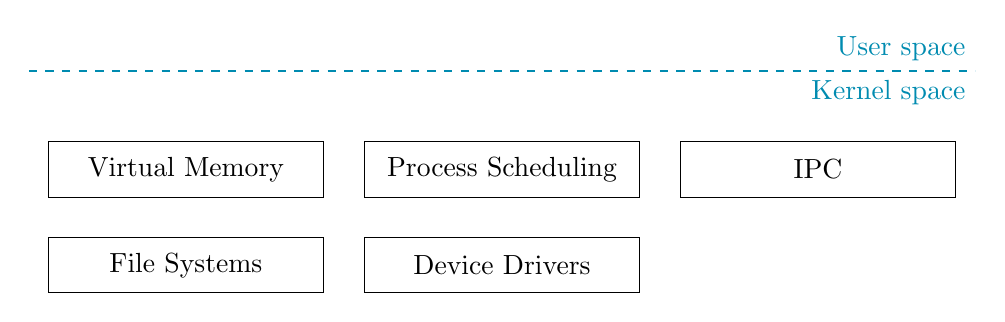
\begin{tikzpicture}[box/.style={draw, minimum width=3.5cm,
                                  minimum height=2em,
                                  inner sep=0.5em, node distance=0.5cm}]
    \draw [blue, dashed, thick] (0,0) -- ($(\textwidth - 3pt, 0)$);
    \node [blue, anchor=south east] at ($(\textwidth - 3pt, 0)$)
          (user) {User space};
    \node [blue, anchor=north east] at ($(\textwidth - 3pt, 0)$)
          (kernel) {Kernel space};
    \node [box] (sched) at ($(\textwidth/2 - 1.5pt, -1.25)$)
          {Process Scheduling};
    \node [box, left=of sched] {Virtual Memory};
    \node [box, right=of sched] {IPC};
    \node [box, below=of sched] (dd) {Device Drivers};
    \node [box, left=of dd] {File Systems};
  \end{tikzpicture}
\end{slide}

\begin{slide}
  
  \slidetitle{A Microkernel Runs the Minimum Amount of Services in Kernel
              Mode}

  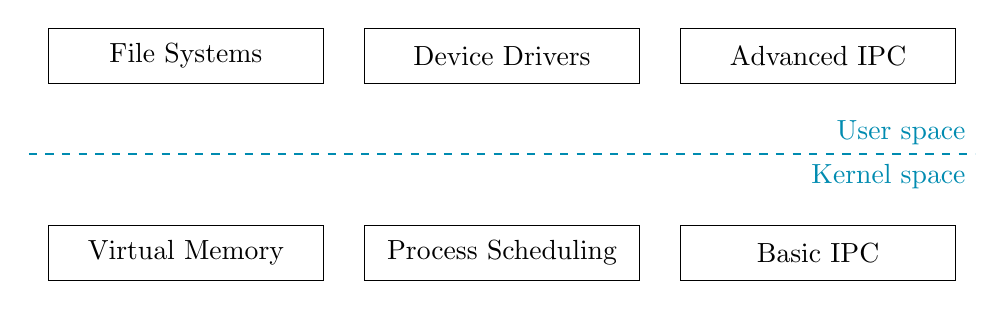
\begin{tikzpicture}[box/.style={draw, minimum width=3.5cm,
                                  minimum height=2em,
                                  inner sep=0.5em, node distance=0.5cm}]
    \draw [blue, dashed, thick] (0,0) -- ($(\textwidth - 3pt, 0)$);
    \node [blue, anchor=south east] at ($(\textwidth - 3pt, 0)$)
          (user) {User space};
    \node [blue, anchor=north east] at ($(\textwidth - 3pt, 0)$)
          (kernel) {Kernel space};
    \node [box] (sched) at ($(\textwidth/2 - 1.5pt, -1.25)$)
          {Process Scheduling};
    \node [box, left=of sched] {Virtual Memory};
    \node [box, right=of sched] {Basic IPC};
    \node [box] (dd) at ($(\textwidth/2 - 1.5pt, 1.25)$) {Device Drivers};
    \node [box, left=of dd] {File Systems};
    \node [box, right=of dd] {Advanced IPC};
  \end{tikzpicture}
\end{slide}

\begin{slide}
  
  \slidetitle{Other Types of Kernels}

  ``Hybrid'' kernels are between monolithic and microkernels

  \leftspace{}Emulation services to user mode (Windows)

  \leftspace{}Device drivers to user mode (macOS)
  \bigskip

  Nanokernels and picokernels

  \leftspace{}Move even more into user mode than traditional microkernels
  \bigskip

  There's different architectural lines you can draw with different trade-offs
\end{slide}

\begin{slide}

  \slidetitle{Kernel Interfaces Operate Between CPU Mode Boundaries}

  The lessons from the lecture:

  \begin{itemize}
    \item The kernel is the part of the OS that interacts with hardware \newline
          (it runs in kernel mode)
    \item System calls are the interface between user and kernel mode
      \begin{itemize}
        \item Every program must use this interface!
      \end{itemize}
    \item File format and instructions to define a simple ``Hello world''
          (in 168 bytes)
      \begin{itemize}
        \item Difference between API and ABI
        \item How to explore system calls
      \end{itemize}
    \item Different kernel architectures shift how much code runs in kernel
          mode
  \end{itemize}

\end{slide}

\end{document}